% $Id: Parameters.tex,v 1.1 2008/01/31 18:04:16 dconway Exp $
\chapter{\label{chapter:Parameters}Calculated Parameters and Stopping Conditions}
\chapauthor{Linda O. Jun}{Goddard Space Flight Center}
\chapauthor{Darrel J. Conway}{Thinking Systems, Inc.}

GMAT contains classes designed to perform numerous data calculations applicable to the analysis of
spacecraft trajectories, orientations, and mission goals.  These calculations are performed by the
Parameter class hierarchy.  This chapter describes, in some detail, the design of these Parameter
classes.

The Parameter classes can be used in conjunction with the propagators to perform precision
propagation, enabling the ability to stop on calculated values provided by the Parameter objects.
Section~\ref{section:StoppingConditions} provides a description of the stopping condition classes.
Stopping conditions are used by the Propagate command, described in Section~\ref{section:Propagate}.

\section{\label{section:Parameters}Parameters}

<<To be completed.>>

\section{\label{section:StoppingConditions}Stopping Conditions and Interpolators}

\begin{figure}[htb]
\begin{center}
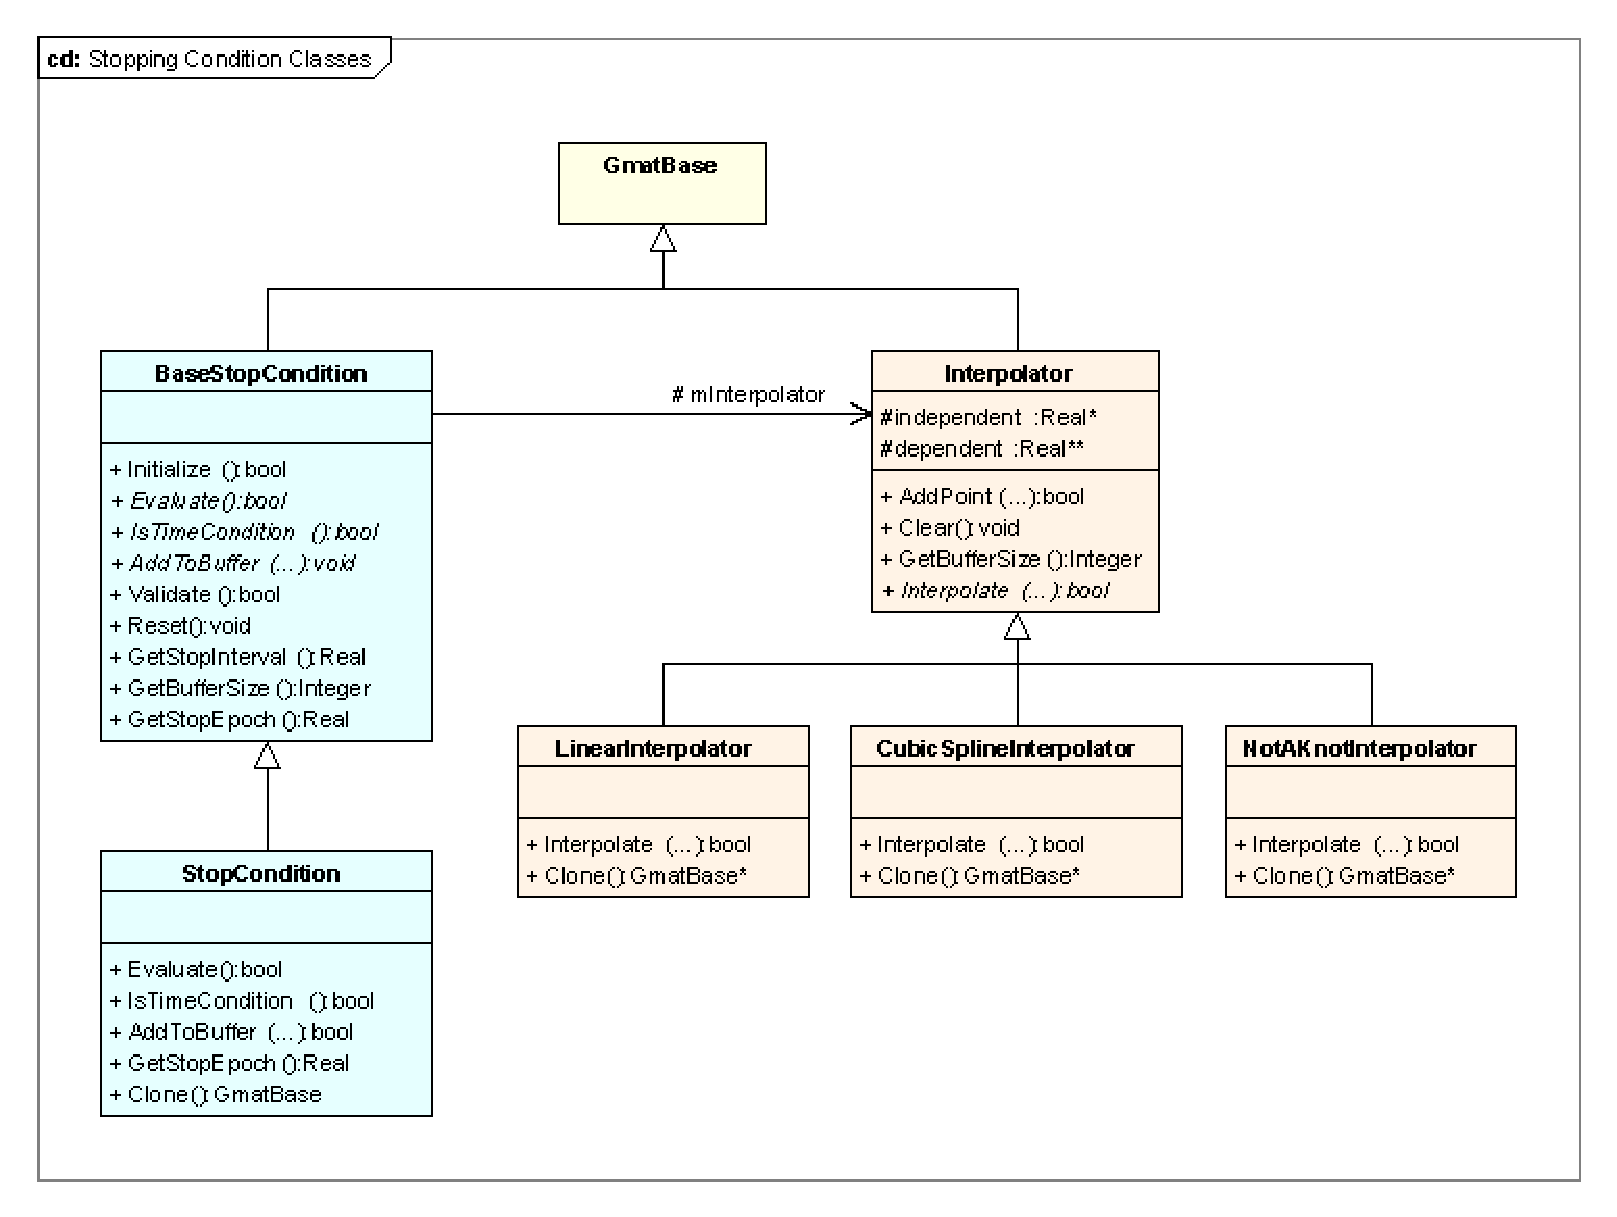
\includegraphics[scale=0.5]{Images/StoppingConditionClasses.eps}
\caption{\label{figure:StoppingConditionClasses}Stopping Condition Classes}
\end{center}
\end{figure}

Propagation in GMAT is described in Section~\ref{section:Propagate}.  The propagation algorthme
described there include descriptions about stopping at specific locations on a SpaceObject's
trajectory, and include a discussion of the use of interpolators for these stopping points.  The
parameters and interpolators used for stopping are encapsulated in the stopping condition classes
and interpolator classes shown in Figure~\ref{figure:StoppingConditionClasses}.  These classes are
described in the following sections.

\subsection{Stopping Conditions}

Stopping conditions are implemented in two classes, as shown in the figure.  These classes are
described below.

\textit{Note: These sections need to be filled in.  There will be some updates as implementation
of the Propagate updates proceed.}

\subsubsection{The BaseStopCondition Class}

\subparagraph{Methods}
\begin{itemize}
\item \textbf{bool Initialize()}
\item \textbf{virtual bool Evaluate() = 0}
\item \textbf{virtual bool IsTimeCondition() = 0}
\item \textbf{virtual void AddToBuffer(bool isInitialPoint) = 0}
\item \textbf{bool Validate()}
\item \textbf{void Reset()}
\item \textbf{Real GetStopInterval()}
\item \textbf{Integer GetBufferSize()}
\item \textbf{Real GetStopEpoch()}
\end{itemize}

\subsubsection{The StopCondition Class}

\subparagraph{Methods}
\begin{itemize}
\item \textbf{virtual bool Evaluate()}
\item \textbf{virtual bool IsTimeCondition()}
\item \textbf{virtual void AddToBuffer(bool isInitialPoint)}
\item \textbf{Real GetStopEpoch()}
\item \textbf{GmatBase Clone()}
\end{itemize}

\subsection{Interpolators}

GMAT implements interpolators using a framework implemented in the Interpolator base class.  Each
derived class uses the Interpolator data structures and methods that implement the data buffers,
add points to them, clear the buffers, and provide buffer size information.  The base class
provides the interface to the call to obtain interpolated data as an abstract method, Interpolate().

\subsubsection{The Interpolator Class}

Interpolator is the base class for all GMAT interpolators.  It implements the data storage and
access functions needed by interpolation routines, and provide the facilities needed to store and
access the data in a ring buffer sized to match the interpolation algorithm.

\subparagraph{Class Attributes}

\begin{itemize}
\item \textbf{Real* independent}: The array of independent data used for interpolation.
\item \textbf{Real** dependent}: The dependent data arrays used for interpolation.
\end{itemize}

\subparagraph{Methods}

\begin{itemize}
\item \textbf{bool AddPoint(Real ind, Real* date)}: Adds independent and dependent data to the
arrays of data elements.  The data is stores in these arrays using a ring buffer allocation, so
that data does not need to be copied when the number of points in the buffer exceeds the allocated
array sizes.  Instead the new data overwrites the oldest values in the arrays.
\item \textbf{void Clear()}:  Resets teh rind buffer pointers, so that the buffers appear to be
empty on their next use.
\item \textbf{Integer GetBufferSize()}:  Returns the number of data points that can be stored in
the ring buffer.
\item \textbf{virtual bool Interpolate(Real ind, Real* results) = 0}: The abstract method that gets
overridden to implement specific interpolation algorithms.
\end{itemize}

\subsubsection{The Linear, Cubic Spline, and Not-a-Knot Interpolators}

GMAT implements three interpolators: a linear interpolator, a standard cubic spline interpolator
using the algorithm described in \cite{recipes}, and the not-a-knot algorithm described in
\cite{mathSpec}.  These classes implement two class specific methods:

\subparagraph{Methods}

\begin{itemize}
\item \textbf{GmatBase* Clone()}:  Calls the class's copy constructor to make an exact copy of the
interpolator.
\item \textbf{virtual bool Interpolate(Real ind, Real* results)}: Implements the specific
interpolation algorithm used by the interpolator.
\end{itemize}

\noindent The Clone method behaves as in all other GmatBase subclasses.  The Interpolate() methods
implement the interpolator specific algorithms, as described in the references.
